% Options for packages loaded elsewhere
\PassOptionsToPackage{unicode}{hyperref}
\PassOptionsToPackage{hyphens}{url}
%
\documentclass[
]{article}
\usepackage{lmodern}
\usepackage{amssymb,amsmath}
\usepackage{ifxetex,ifluatex}
\ifnum 0\ifxetex 1\fi\ifluatex 1\fi=0 % if pdftex
  \usepackage[T1]{fontenc}
  \usepackage[utf8]{inputenc}
  \usepackage{textcomp} % provide euro and other symbols
\else % if luatex or xetex
  \usepackage{unicode-math}
  \defaultfontfeatures{Scale=MatchLowercase}
  \defaultfontfeatures[\rmfamily]{Ligatures=TeX,Scale=1}
\fi
% Use upquote if available, for straight quotes in verbatim environments
\IfFileExists{upquote.sty}{\usepackage{upquote}}{}
\IfFileExists{microtype.sty}{% use microtype if available
  \usepackage[]{microtype}
  \UseMicrotypeSet[protrusion]{basicmath} % disable protrusion for tt fonts
}{}
\makeatletter
\@ifundefined{KOMAClassName}{% if non-KOMA class
  \IfFileExists{parskip.sty}{%
    \usepackage{parskip}
  }{% else
    \setlength{\parindent}{0pt}
    \setlength{\parskip}{6pt plus 2pt minus 1pt}}
}{% if KOMA class
  \KOMAoptions{parskip=half}}
\makeatother
\usepackage{xcolor}
\IfFileExists{xurl.sty}{\usepackage{xurl}}{} % add URL line breaks if available
\IfFileExists{bookmark.sty}{\usepackage{bookmark}}{\usepackage{hyperref}}
\hypersetup{
  pdftitle={Response to reviews},
  hidelinks,
  pdfcreator={LaTeX via pandoc}}
\urlstyle{same} % disable monospaced font for URLs
\usepackage[margin=1in]{geometry}
\usepackage{graphicx,grffile}
\makeatletter
\def\maxwidth{\ifdim\Gin@nat@width>\linewidth\linewidth\else\Gin@nat@width\fi}
\def\maxheight{\ifdim\Gin@nat@height>\textheight\textheight\else\Gin@nat@height\fi}
\makeatother
% Scale images if necessary, so that they will not overflow the page
% margins by default, and it is still possible to overwrite the defaults
% using explicit options in \includegraphics[width, height, ...]{}
\setkeys{Gin}{width=\maxwidth,height=\maxheight,keepaspectratio}
% Set default figure placement to htbp
\makeatletter
\def\fps@figure{htbp}
\makeatother
\setlength{\emergencystretch}{3em} % prevent overfull lines
\providecommand{\tightlist}{%
  \setlength{\itemsep}{0pt}\setlength{\parskip}{0pt}}
\setcounter{secnumdepth}{-\maxdimen} % remove section numbering

\title{Response to reviews}
\author{}
\date{\vspace{-2.5em}}

\begin{document}
\maketitle

\emph{italics - temporary comments for points that remain to be
addressed}

\textbf{bold - response}

\textasciitilde\textasciitilde\textasciitilde\textasciitilde{}

Dear Editor:

\ldots{} Major changes included the following:

\begin{itemize}
\item
  At the request of 3 reviewers (R1,R3,R4), we tried an alternate metric
  of drought resistance (using an ARIMA model to project what growth
  would have been in drought year based on the trend over the past 10
  years). Results were similar, and we now present that as a secondary
  model (mostly in SI).
\item
  We slightly modified the method of determining which trait variables
  go into the full model. Specifically, we added the criteria of
  consistent direction across droughts, and as a result dropped xylem
  porosity. This also makes sense because the two diffuse porous species
  (Liriodendron tulipifera and Fagus grandifolia) are at opposite ends
  of the spectrum in terms of drought resistance. (Side note: this
  contradicts the current understanding that diffuse porous species in
  the temperate deciduous biome are more drought sensitive, but not the
  bigger global picture, as R2 points out.).
\item
  We moved former tables 4 and 5 to the SI.
\item
  We added two figures: one showing Rt differences across species, and
  one visualizing the model results (the latter is not yet right, as
  gg-plot is being difficult, but will eventually match the model
  results.)
\end{itemize}

The result is an easier to read paper with more robust support.

\newpage

\hypertarget{referee-1}{%
\subsection{Referee: 1}\label{referee-1}}

Comments to the Author

The study addresses the relationship between drought resistance (Rt)
calculated from radial growth, and different traits and
microenvironmental characteristics on 12 tree species from one forest in
the Eastern US. Both the dataset and the study are meaningful, and the
relationship found between Rt and height of biological importance.
However, I think there are a number of issues that need to be worked
out.

It is important to better discuss the proper use of Rt, particularly
when comparing single drought years, to assess tree resistance to
drought. This metric has been much used lately as one of the so-called
resilience indices (I wonder why other Rs indices where not included in
the manuscript). In the paper, the authors use Rt similarly to most
studies in the literature, which is fine. Yet, Rt (and particularly the
other resilience indices based on radial growth) does not only depend on
the individual response to drought events, but also on stand dynamics
around target trees. For this reason, if stands around trees are not
comparable or show changes after some disturbance (e.g.~the drought
events analysed) differently, this may bias comparisons of Resilience
indices (although it is true that Rt should be less influenced than the
other indices). The problem is that there is not such stand competition
data for old droughts. This does not invalidate the study but I think
the authors should discuss the issue, particularly for the analysis and
comparisons of single droughts. I would suggest including also other
Resilience indices, not only Rt, to enrich the discussion.

\href{https://github.com/SCBI-ForestGEO/McGregor_climate-sensitivity-variation/issues/92}{\emph{issue
\#92}}

\textbf{To account for potential trends in individual tree growth prior
to the drought, which could be influenced by stand dynamics, we tried an
intervention time series analysis (ARIMA). Details on the comparison
between \(Rt\) and \(Rt_{ARIMA}\) are presented in the responses to
reviewer 4. In short, the ARIMA method yielded broadly similar results,
but tended to produce less reasonable estimates when the difference
between the two metrics was large, so we decided to retain \(Rt\) as the
focal metric. While this unquestionably leads to biased estimates for
some trees, we would not expect it to bias our analysis; rather, it is
one of the reasons that the amount of variation that can be explained by
analyses such as these is relatively low. We now include the following
content on ARIMA in the manuscript:}

(\emph{insert text})

\textbf{Regarding the resilience indices, we considered analyzing these
and decided it would be best to stick with just resistance for three
reasons: (1) Most importantly, we would expect resilience to be governed
by fundamentally different mechanisms than resistance. While it would be
interesting to examine resilience, this would be beyond the scope of the
current paper. (2)
\href{https://www.nature.com/articles/s41467-020-14300-5}{DeSoto et
al.~(2020, Nature)} used an extensive dataset of trees sampled after
severe droughts and compared the responses to previous, less-severe
droughts between trees that survived and trees that were killed by the
severe drought. In angiosperms, trees that died from a severe drought
had lower resistance to previous droughts, compared to trees that
survived the severe drought. In gymnosperms, trees that died during
severe droughts had lower recovery following previous droughts, compared
to trees that survived the severe drought. These findings would argue
that resistance is a more important variable for angiosperms. (3) As the
reviewer notes, resilience indices would probably tend to be more
sensitive to a tree's neighborhood and prior conditions. We now state
the logic for focusing on \(Rt\) in the methods section:}

\textbf{``We focus exclusively on drought resistance (\(Rt\) or
\(Rt_{ARIMA}\)), and not on the resilience metrics described in Lloret
\emph{et al.} (2011), because (1) we would expect resilience to be
controlled by a different set of mechanisms, and (2) the findings of
\emph{\href{https://www.nature.com/articles/s41467-020-14300-5}{DeSoto
et al.~(2020)}} suggest that \(Rt\) is a more important drought response
metric for angiosperms.''}

Statistical analysis: the analysis would be more precise if the authors
used Generalized linear mixed models to avoid data transformation and
take into account (with random effects, as they do for the linear mixed
model, LMM, presented now) the influence of species in the analysis.
Then I missed a further discussion on the role of individual species
(e.g.~see my comment below on Rt\textgreater1).

\textbf{A GLMM would only avoid transformation of the dependent variable
(Rt), but that was (and is) not transformed. We tried the analysis with
generalized linear mixed models with a Gaussian distribution, and
confirmed that this gave very similar results, so we are sticking with
LMM.}

I suggest to show some relationship, e.g.~between Rt and traits in
figures. The study only presents two figures and there is plenty of room
to present results more clearly with extra figures.

\textbf{We created a new figure (\emph{Fig. 4}) visualizing the top
model results.}
(\href{https://github.com/SCBI-ForestGEO/McGregor_climate-sensitivity-variation/issues/71}{\emph{issue
\#71}}()

\textbf{We have \emph{also} added a new figure (\emph{Fig. 2}) showing
how \(Rt\) varied across species in each of the three droughts.}

Only assessing models with AIC is not enough to prove sound
relationships in multidimensional and complex data-models. LL ratio
tests or deviance-anova tests can be used in the case of nested models
with LMM or GLMM respectively. Along the text: dAIC is generally
referred as \(\Delta\)AIC, please change accordingly.

\href{https://github.com/SCBI-ForestGEO/McGregor_climate-sensitivity-variation/issues/94}{\emph{issue
\#94}}

\textbf{We have gone through the manuscript / tables and figures and
updated where it said ``dAICc'' to be \(\Delta\)AICc. }

Following the two previous comments, I suggest to leave in Table 5 just
the best model (rather that a multimodel inference as is presented now)
to discuss more clearly the covariates included. And I suggest
discussing only the model with all years together. This would be more
robust and avoid ramble differences between years that mostly look
spurious and with a difficult physiological explanation. This would help
to ensure a better use of the Resilience indices.

\textbf{In the spirit of this comment (simplifying presentation), we
have created a new figure (\emph{Fig. 4}) visualizing the results of the
best model. We moved Table 5 to the Appendix (now Table S6, plus a
parallel Table S7 for \(Rt_{ARIMA}\)).}

\textbf{We have also dramatically decreased the emphasis on differences
across drought years, as follows:* }

\textbf{(1) Table 1 now shows just the results from the model with all
drought years combined.}

\textbf{(2) The results and discussion now focus on the results from the
three drought years combined.}

\textbf{(3) In order to make models more consistent across years and
reduce spurious correlations, we now include the criteria that for a
trait to be included as a candidate variable in the full model, the sign
of coefficients must be consistent across all droughts (in addition to
meeting the AIC criteria, as before). This resulted in only two
candidate variables for the main model (\(PLA_{dry}\) and
\(\pi_{tlp}\)). (Removed was ring porosity, which had opposite effects
in different droughts.)}

\emph{We do plot the three droughts separately in figures
\textbf{\#,\#}, as we do fee that this makes the story richer.}

The authors might like to consider including Table 4 as a supplement,
because as it stands it looks like an exploratory analysis. If the
`single-variable approach' is not just exploratory, state it clearly and
why it is needed besides the full models with several parameters.

\textbf{We have moved this table to the SI. We modified the analysis
approach such that separate models for individual variable tests (as
previously show in this table) are now limited to the species traits.
While this table is (and was) the only display item (besides Table 1)
giving these results, the results are either mostly negative (wood
density, SLA, xylem porosity) or preliminary tests qualifying variables
for inclusion in full model (\(PLA_{dry}\) and \(\pi_{tlp}\)).}

Importantly, the drought selection would be biased if years were
selected as from line 202, which is a common mistake in similar studies
(the original of Lloret et al.~included). Droughts must be selected
based only on some climatic/drought index (PDSI, SPEI,\ldots) and
independently of growth. Otherwise the analysis is biased towards years
with low growth, and different questions would arise with a difficult
answer. If the authors select only those droughts where there is a
growth decrease: is that decrease evident in all species and similar
across species? What happens with more intense droughts that those
selected (if any), why they do not force a decrease in growth if drought
is a main forcing agent? I see that 1966 and 1999 are the driest (as in
PDSI) in Figure 1, but there is at least one year around 1955 that it is
as dry or drier than 1977. In line 204 it is stated that they are the
driest. If this is the case, the analysis should be sound but it should
be deleted what is stated in lines 202-203 where authors say that they
selected years also based on low growth. In fact, that should be a
result after having selected the drought years only based on dryness (as
in lines 208-209). Line 211 then they search for pointer years\ldots{} a
little bit messy. Please, explain better, and it should follow: 1)
selection of dry years without regarding growth data; 2) characterise
growth those dry years; 3) If the authors want to compare with other
pointer years, fine, but that should be a third independent step
properly justified and explained. Following this rationale, then in line
221 it should be difficult that Rt\textgreater1, had we selected those
years with a negative growth anomaly. Please, explain clearly and
consistently.

\textbf{We have made the suggested change: we now present only the PDSI
criteria in the methods, and mention the fact that the selected years
were also the ones with largest growth reductions during the study
period in the results section. Using just the PDSI criterion does not
change the years analyzed.}

Other minor comments:

\begin{itemize}
\tightlist
\item
  Line 113: correct `positively'.
\end{itemize}

\textbf{done}

\begin{itemize}
\tightlist
\item
  Line 134: cambial growth also includes that of phloem; so better refer
  to `xylem growth'.
\end{itemize}

\textbf{done}

\begin{itemize}
\tightlist
\item
  Line 161: how many species were estimated for height like this?
  Wouldn't it be possible for authors to go to the field and perform
  some height estimations? This should be rather straightforward and the
  authors would increase accuracy across species in height estimation.
\end{itemize}

\textbf{We have specified how many species used the interspecific
allometry (n=2, JUNI and FRAM). Because of COVID-19, it would not be
possible to go collect more data for these species.}

\begin{itemize}
\tightlist
\item
  Lines 166-167: please explain further the hypothesis and why.
\end{itemize}

\textbf{We have reworded this sentence to read, ``While some tree crowns
undoubtedly changed position over the past several decades, in this case
the bias would be unlikely to result in false acceptance of the
prediction that dominant trees have the lowest \(Rt\) (\emph{i.e.}, type
I error unlikely, type II error possible), making our hypothesis test
conservative.''}

\begin{itemize}
\tightlist
\item
  Line 222: what about climate in years before 1991?
\end{itemize}

\textbf{We no longer mention 1991, as it does not meet the PDSI
criteria.}

\begin{itemize}
\tightlist
\item
  Line 231: define AICc.
\end{itemize}

\textbf{This is done (with added reference)}

\begin{itemize}
\tightlist
\item
  Line 234-247: it is not clear what the authors did, please explain
  clearer this paragraph and the next and why you did two different (yet
  similar) analyses (single-variable and full model).
\end{itemize}

\textbf{This section has been re-written.}

\begin{itemize}
\tightlist
\item
  Line 241-242: enough to say once that models were selected based on
  AIC (line 237-238) and then one criterion, why dAIC\textless1 here and
  dAIC\textless2 before? The classic assumption is 2 (e.g.~Burnham \&
  Anderson 2004). See also my other comment above.
\end{itemize}

\textbf{We have modified this text to read as follows:}

\textbf{``Trait variables were considered appropriate for inclusion in
the main model if they had a consistent direction of response across all
droughts and if their addition to a corresponding null model lacking the
trait improved fit (at \(\Delta\)AICc \(\ge\) 1.0) in at least one
drought year (Table 4). We note that the \(\Delta\)AICc \(\ge\) 1.0
criterion is not a test of significance, but of whether the variable has
enough influence to be considered as a \emph{candidate} variable in full
models.''}

\begin{itemize}
\tightlist
\item
  Line 255-256: but this was already an assumption in M-M (line
  202-203). Please, see my comment below and be consistent along the
  text.
\end{itemize}

\textbf{As stated above, we have removed the \(Rt\) criterion from the
drought identification process, and now present this information for the
first time in this section, adding the following statement: ``Across the
entire study period (1950-2009), the focal drought years were the three
years with the largest fraction of trees exhibiting \(Rt \le 0.7\).''}

\begin{itemize}
\tightlist
\item
  Line 258: so this means that they are no sensitive to the drought?
  Which trees, any species in particular? Is this a consequence of stand
  dynamics shadowing the impact of drought events?
\end{itemize}

\textbf{It's not unprecedented to see some trees exhibit increased
growth during drought, and not surprising. Stand dynamics and other
factors result in a lot of scatter in the relationship between tree
growth and climate, so while the distribution of \(Rt\) in Fig. 1b was
shifted left (normal year should be normally distributed around 1),
there still are some trees with increased growth. Our analysis helps to
work out which trees these were (often shorter trees).}

\textbf{We address this question in the discussion, where we have added
a statement about how this is not unprecedented: ``Across all three
droughts, the majority of trees experienced reduced growth, but a
substantial portion had increased growth (Fig. 1b), potentially due to
decreased leaf area of competitors during the drought, and consistent
with prior observations that smaller trees can exhibit increased growth
rates during drought (Bennett et al.~2015). It is likely because of the
moderate impact of these droughts, along with other factors influencing
tree growth (e.g., stand dynamics), that our best models characterize
only a modest amount of variation''}

\textbf{We have also added a new figure (\emph{Fig. 2}) showing how
\(Rt\) varied across species in each of the three droughts.}

\begin{itemize}
\tightlist
\item
  Line 266-267: why only in 1966? I think this shows that this variable
  is not properly assessed. The older the date, the more accurate the
  estimation of crown position and height were.
\end{itemize}

\textbf{It is true that crown position estimates become more accurate in
later dates, but height should be equally reliable across years, having
been estimated based on reconstructed DBH. This was not previously
clearly specified in the methods. To clarify, we have added the
following statement: ``We then used these allometries to estimate \(H\)
for each drought year, \(Y\), based on reconstructed \(DBH_Y\).''}

\textbf{We agree that the assessment of crown position is somewhat
problematic, both because of its increasing inaccuracy going back
through time, and because of collinearity with \(H\). However, given
that it is both biologically interesting and comes out in our top
models, we have chosen to include it. We note that this makes the test
of our hypothesis conservative. We are transparent about this issue, to
which we devote a paragraph in the discussion (par. 3).}

\emph{see issue on CP!!!!}

\begin{itemize}
\tightlist
\item
  Line 275-280: those profiles were assumed a priori in the introduction
  and are common to any forest. They are indeed interesting to
  characterise the forest, but they do not add to individual tree
  variability. You could think to send Figure 2 to an appendix, in
  consequence, and use figures to show more specific results related to
  your individual tree analyses.
\end{itemize}

\textbf{Our preference is to keep this figure in the main manuscript. We
agree that similar patterns are common to any forest, and are not trying
to claim this as any kind of novel result, but we're not aware of
studies showing similar height profiles for a temperate forest. Such
patterns are not shown some relevant textbooks: Gordan Bonan's 2016
\emph{Ecological Climatology} and Norman \& Campbell's
\emph{Environmental Biophysics}. If we're missing studies that show such
vertical profiles, we'd appreciate the references.}

\textbf{We did create two new figures showing the results of the
tree-ring analysis (and moved two tables to the SI).}

\begin{itemize}
\tightlist
\item
  Line 330-331: any evidence to support this? It looks rather
  speculative. As suggested above, does any species particularly show
  positive Rt or positive Rt are randomly distributed in your trees?
\end{itemize}

\emph{Current text, with phrase of concern in bold: ``Across all three
droughts, the majority of trees experienced reduced growth, but a
substantial portion had increased growth (Fig. 1b), potentially due to
decreased leaf area of competitors during the drought (\textbf{REF--if
we can find one}), and consistent with prior observations that smaller
trees can exhibit increased growth rates during drought (Bennett
\emph{et al.}, 2015).'' }

\textbf{To address the question about species, we have added a new
figure (\emph{Fig. 2}) showing how \(Rt\) varied across species in each
of the three droughts.}

\begin{itemize}
\tightlist
\item
  Line 331-333: not so sure about this. It can also mean that there is
  no causal relationship between Rt and covariates, mostly because
  radial growth Rt should not be used as an integral proxy of tree
  resistance to drought, such as it is often used now in the literature.
\end{itemize}

\emph{Tree-ring data inherently have a lot of variation. Neil could
probably write a better response here, with refs.}

\begin{itemize}
\tightlist
\item
  Line 334-339: indeed, assessment of these two variables is not
  conclusive, as suggested above (just data from 2018, from the past
  estimated and correlated).
\end{itemize}

\textbf{Please see response above.}

\begin{itemize}
\tightlist
\item
  Line 348: non-drought.
\end{itemize}

\textbf{Fixed.}

\begin{itemize}
\tightlist
\item
  Line 349: do authors really think that lower radial growth as from Rt
  on a specific year means that the tree is more vulnerable? I think
  this is over conclusive.
\end{itemize}

\textbf{We did not intend the meaning here as vulnerability \emph{to
mortality} (assuming that's the objection here). We have reworded this
sentence to read, ``Belowground, taller trees would tend to have larger
root systems, but the potentially greater access to water did not
override the disadvantage conferred by height--and, in fact, greater
moisture access in non-drought years (here, higher TWI) appears to make
trees more sensitive to drought (Zuleta \emph{et al.}, 2017; Stovall
\emph{et al.}, 2019).''}

\begin{itemize}
\tightlist
\item
  Line 400: I do not agree we can directly link Rt with tree
  vulnerability to drought; we might be currently overinterpreting these
  resilience indices extrapolating to physiological conclusions that do
  not necessary need to hold.
\end{itemize}

\textbf{See above comment. We have reworded this sentence to read, ``In
the meantime, the results of this study advance our knowledge of the
factors conferring drought resistance in a mature forest, opening the
door for more accurate forecasting of forest responses to future
drought.''}

Table 1: do `-` signs in the table correspond to `no' (non-significant)?
Please explain.

\textbf{This is now clarified in the table footnote.}

Table 3: please, add also the number of trees, it is more informative
than the number of cores to check sample size in your study.

\textbf{In this study, we have one core per tree, now specified in the
methods. We have changed the table header to ``n trees''.}

Table 3: the authors could show some test to see if the traits presented
are different among species.

\textbf{We now show differences in traits among species in Table S4.}

\emph{need to add ANOVA, prsent reults in paper}

Table S1 and S2: correct R2.

\emph{IM I added the correct Latex notation but it's not rendering it
when I knit the file\ldots{} (KAT: I just tried and wasn't able to get
it working.}

Table S3: please, explain what `rank' means.

\textbf{Done.}

Figure S3: I understand that authors only have height data from 2018 and
height for the other dates looks trivial: indeed there will be an
increase in height with an increase in DBH in time. The question is
whether there was any stand dynamics involved in those height series
that had to be included in the models.

\textbf{We recognize the importance of stand dynamics, and have added
specific mention to the discussion: ``It is likely because of the
moderate impact of these droughts, along with other factors influencing
tree growth (e.g., stand dynamics), that our best models characterize
only a modest amount of variation,\ldots{}''}

\hypertarget{referee-2}{%
\subsection{Referee: 2}\label{referee-2}}

Comments to the Author

This manuscript examines a truly urgent and important issue. The general
issue is the clear vulnerability of forests to ongoing climate change
induced drought worldwide. The issue is particularly vexing because,
while it seems clear that plant hydraulics is involved in vulnerability
to drought, the exact mechanisms connecting hydraulics to vulnerability
are not clear, and just what indices biologists should use to gauge
vulnerability is as a result unclear. Within the broad pattern of global
forest decline with climate change induced drought is the particularly
mystifying and horrific preferential loss of the largest individuals all
over the world. In addition to their esthetic appeal, large individuals
make disproportionate contributions to forest function, making the issue
examined in this ms extremely timely and important.

The issue of the preferential death of large trees is not only important
because of its effects on forest function and culture. It is important
because it seems to require novel theory. Under current expectations,
the largest individuals, with their greater root reach, etc., should be
more rather than less resistant. That they might not be demands a novel
explanatory framework. Yet the very existence of the tendency is
debated, with some studies reporting greater mortality among small
rather than large individuals (Camarero et al., 2015; Colangelo et al.,
2017). These studies, however, were not designed to take into account
the microsite variation that presumably should lead to marked
differences in survivorship even within the same height class with
drought. One approach, which we have used (Soriano et al., in press;
Olson et al., 2018) is to conduct experiments under controlled
conditions to detect the effect of height, and our results are
consistent with the greater vulnerability of taller individuals.
However, under natural conditions, a study that takes this variation
into account is needed to test the notion that taller individuals are
preferentially vulnerable is needed, and this study provides exactly
such a design.

I found this paper not only to address a very important point but also
to be exceptionally well structured and written. My main suggestion is
that it could use a bit more emphasis on its importance, and I would be
interested in hearing a bit more about what the authors feel their
results imply regarding the cause of the preferential vulnerability of
large individuals. I give line-by-line suggestions (and sometimes just
reactions):

\textbf{Thank you for this wonderful review.}

\emph{What a nice review! We can easily add some language on the
importance. We should also add citations to many of the studies
mentioned.}

first paragraph---this setup is very compelling, and the point is
urgently true.

\textbf{Thank you}

66- ``in their basal portions'' seems fine for this level of intro, but
note that in angiosperms, taller trees also have wider vessels at the
stem tip (and thus throughout the conductive system) (Zach et al., 2010;
Olson et al., 2014, 2018). This seems plausibly the result of selection
keeping conduit carbon costs down with height growth. As a tree grows
taller, if terminal twig vessel diameters become wider, then given a
constant rate of tip-to-base vessel widening, vessel diameters will be
wider along the entire stem. Vessels that are wider throughout would
have lower per-conduit resistance than those that, all else being equal,
are narrower. So, conceivably as a tree gets taller, if vessels widen at
the twig tip, then lower per-conduit resistance could mean that the same
leaf area is supplied by fewer vessels. This could potentially
contribute to keeping per-leaf area carbon costs constant with height
growth. This prediction seems confirmed by the experiment of (Echeverría
et al., 2019), who found that as Moringa trees grew taller, there were
wider vessels at the stem tip and fewer vessels per unit leaf area, but
that conductance per unit leaf area should remain the same. Terminal
twig tracheids don't seem to widen in gymnosperms, e.g.~(Williams et
al., 2019). (Sack et al., 2012) have shown very clearly that petiole
base vessel diameter scales predictably with leaf size, as would be
expected; it is not clear how leaf size variation is involved in
terminal twig vessel diameter scaling with height, though in wide
samplings leaf size doesn't seem to scale with height (Jensen \&
Zwieniecki, 2013).

\textbf{Thank you for this interesting information. We've modified the
sentence to read, "Indeed, tall trees require xylem of greater hydraulic
efficiency, such that xylem conduit diameters are wider in the basal
portions of taller trees, both within and across species (Olson \emph{et
al.}, 2018; Liu \emph{et al.}, 2019), and throughout the conductive
systems of angiosperms (Zak et al.~2010, Olson et al.~2014,2018).}

67 Appealing to the vulnerability-diameter link might get blowback from
some readers because there is as yet no satisfactory theory linking
vulnerability to diameter in an entirely satisfactory way, so maybe just
say ``wider conduits are likely'' or that they are ``plausibly'' or
``possibly'' more vulnerable, or that many ``data are consistent'' with
such a link. My view is that there very well might not be a link, but in
the absence of a link between vulnerability and conduit diameter, it is
very hard to explain a very large number of well-established
observations. These include the following: why growth rings always
proceed from wide to narrow conduits as drought ensues; why maximum
community conduit diameter is narrower in drylands than in wet places;
why lianas have wider vessel diameter variances (i.e.~not only wider but
also numerous narrower vessels) than self-supporting plants (Rosell \&
Olson, 2014); why plants virtually always produce vessels narrower than
the maximum possible; when internal helical sculpture in conduits varies
in a growth ring it is always associated with narrow latewood vessels;
when simple and scalariform plates vary across growth rings sclariform
plates are always found in the narrow latewood vessels; and many other
observations. If there is no link between drought induced embolism
vulnerability and conduit diameter, and there might not be, all of these
observations, which are currently simultaneously and parsimoniously
explained by the link, will require alternative explanations. As a
result, while there is as yet no well accepted mechanistic link between
vulnerability and diameter, it seems to me irresponsible to reject the
link without providing a satisfactory and similarly parsimonious and
general replacement explanation for all of these phenomena. So, I think
the authors are justified in cautiously invoking the link here.

\textbf{We've added the word ``plausibly''. We agree that this linkage
makes a lot of sense.}

69 this is a very important point---microsite is crucial both for the
ultimate height an individual grows to as well as its vulnerability. The
generalization that on a global level large trees seem
disproportionately vulnerable is often greeted with the skeptical
observation that in specific cases a small tree died next to a large one
that survived. However, the prediction is that \emph{all else being
equal} large individuals should be more vulnerable than smaller
\emph{conspecifics}. There is so much variation in microsite and other
factors that the greater vulnerability of larger individuals should
emerge clearly only in carefully controlled experiments where all else
is indeed (virtually) equal, or with high sample sizes where variation
in microsite etc should random out and the signal of generally higher
vulnerability should come through.

\textbf{Thank you.}

73 The ``greater root reach'' point is almost universally appealed
to---cites for these counterarguments would be useful.

73 Also, larger trees would necessarily seem to have greater stem
storage capacity and thus, if capacitance really is important, more
water volume available for buffering transient drought events, so this
is another reason to expect larger individuals to be more rather than
less resistant.

77 In the concluding sentence, ``greater growth reductions'' came as a
surprise because I thought that the focus was greater vulnerability/
mortality. Also, there are convincing theoretical and empirical reasons
to think that large trees don't slow down e.g.~(Sillett et al., 2010;
Selaya \& Anten, 2010; Michaletz et al., 2014).

96 this all seems compelling. To make the point stronger, either justify
that the leaf traits are causally more important, or that, while they
make up part of a unified hydraulic system all of whose components are
important, leaf traits are simply easier to measure and this justifies
their study. The latter position seems most plausible to me.

102 great questions, though within-species comparisons are likely to be
most informative here, and your mixed model design is in accord with
this; just being cautious because sometimes it's seductive to regard
selection acting between rather than within species

\textbf{Thank you.}

105 this sounds great, but was a little unclear. When you say ``first,
we test\ldots{}'' I thought that you would examine a relationship
between microsite and some tree characteristic, e.g.~that the largest
trees are in moist microsites. But the next sentence didn't refer to a
tree-microsite correlation but vulnerability-size. It would be good to
clarify the prose here because these are very important passages. The
third sentence did seem to be about tree-microsite correlations.

112 wasn't clear where the ``ring porous more drought resistant''
hypothesis came from. Global data show that ring porous species are
almost entirely restricted to the north temperate zone, especially
deciduous broadleaf forests (Wheeler et al., 2007). They are virtually
absent in drylands, especially warm tropical drylands. Species in
drylands are almost overwhelmingly diffuse porous; the high wood density
species in chaparrals and in some desert plants can be semi ring porous
(Olson et al., in press).

\textbf{This is a great point. The hypothesis refers to temperate
deciduous biome, which we now clarify in the sentence in question:}

\textbf{``Studies in temperate broadleaf forests have observed that
ring-porous species showing higher drought tolerance than diffuse-porous
species (Kannenberg \emph{et al.}, 2019; Friedrichs \emph{et al.}, 2009;
Elliott \emph{et al.}, 2015), but this distinction would not hold in the
global context (\emph{Wheeler et al.~2007, Olson et al.~2020}) and does
not resolve differences among the many species within each category.''}

\textbf{We dug into the ring/diffuse porous distinction more, and ended
up making a few substantive changes that relate to this theme: (1) We
added a new figure showing \(Rt\) across species (Fig. 2). This
illustrates that the two diffuse-porous species, \emph{Liriodendron
tulipifera} and \emph{Fagus grandifolia}, were at opposite ends of the
\(Rt\) spectrum. (2) We modified the criteria of selecting candidate
variables for the full models to include the criterion that directions
of responses must be consistent across droughts for inclusion in the
full model. This resulted in exclusion of xylem porosity (Table S4)--a
change that is also warrented by the fact that we only have two
diffuse-porous species. (3) We added the following content to the
discussion: }

\emph{insert text}

113 These correlations seem reasonable, e.g.~see (Méndez-Alonzo et al.,
2012)

124 and Table 3. This seems like a good palette of species because they
are very different in their hydraulic construction. In addition to
libriform fibers, oaks have very abundant vasicentric tracheids,
especially in latewood. This means that the oaks will likely maintain
some conductance even under highly negative tensions. This is not by
virtue of their ring porosity (note that most oaks globally aren't ring
porous!), but because of the high proportion of vasicentric tracheids in
their latewood. Liriodendron (diffuse porous, scalariform perforation
plates) and Carya (likely ring porous at your locality; simple
perforation plates) both have libriform fibers and lack vasicentric
tracheids. See the data in (Olson et al., in press). There is relatively
low family-level diversity represented here; our phylogenetic analyses
(Olson et al., in press) suggest that there is very little phylogenetic
signal in the conduit diameter-stem length relationship, so this could
help justify if necessary not including phylogeny in the analyses.

\emph{this is new terminology to me. Look into Olson et al.~in press.
Would these wood traits be worth including as covariates?}

127 ``tree size''= height?

138 you might discuss the adequacy of the height range studied. If it is
true that conduit diameter predicts vulnerability, then the greatest
differences in vulnerability should be over the height range over which
conduit diameter changes most rapidly. The relationship between conduit
diameter and plant height turns out to follow a power-law like
distribution, see for example the SI in (Olson et al., 2018). This means
that differences in vulnerability should be very marked across smaller
size classes (say below 7 m or so and very marked below 3 m) and be less
and less visible across larger plants. So, studies of changes in conduit
diameter/ vulnerability with height would ideally include plants smaller
than those included here, so maybe comment on how the height range might
affect the ability to detect the patterns of interest. It strikes me
that it is appropriate because it is the height range over which the
putative preferential susceptibility of large trees to drought is being
observed.

173 TWI seems like an appropriate index for characterizing microsite,
with the expectation that individuals in moister areas should be more
buffered from drought.

\textbf{Thank you.}

209 It couldn't hurt to define basal area increment

227 the nesting seems appropriate and sufficient for taking species/
``phylogeny'' into account

260 amazing

\textbf{Thank you.}

275---some people think that the increase in terminal twig vessels with
height growth keeps pace with the changes in VPD from understory to
canopy

281 nice

\textbf{Thank you.}

301 this intro paragraph to the discussion ranks very well the results
from most significant to least

\textbf{Thank you.}

327 I agree that this is the point that most deserves discussion in
paragraph 2

334 You might go into detail regarding what you think this says about
the causal hypothesis behind the global decline of large individuals. To
me it helps reject notions that somehow larger trees are more exposed to
wind throw or other damaging agents. It is consistent with the
hypothesis that larger individuals have wider conduits, and (assuming
that wider conduits are more vulnerable to drought induced embolism)
thus larger individuals are (all else being equal\ldots) more vulnerable
to embolism than smaller conspecifics.

336 beautifully said ``impossible for trees to e ciently transport water
to great heights and simultaneously maintain strong resistance and
resilience to drought-induced embolism''

\textbf{Thank you.}

349 fascinating; it seems plausible that current climate changed induced
large-individual mortality involves trees growing to conduit diameters,
and thus heights, permitted under previously more even and moister
climates, and now finding themselves in more extreme climates that make
their heights and conduits excessively wide given current conditions.

350 if you wanted to expand your discussion of causal mechanisms or the
implications of your findings, I think you could jettison this
paragraph. I admire your thoroughness in offering caveats, but I agree
that this does not seem like a serious problem for your study.

382 an effort that seems in harmony with these concerns is
(Christoffersen et al., 2016)

385 very nice paragraph

\textbf{Thank you.}

In conclusion, this ms addresses a very important issue with a
well-designed study and appropriate analyses. It is well written and
interesting and I hope my comments are useful.

\textbf{Thank you.}

Mark Olson
\href{mailto:molson@ib.unam.mx}{\nolinkurl{molson@ib.unam.mx}}

Camarero JJ, Gazol A, Sangüesa-Barreda G, Oliva J, Vicente-Serrano SM.
2015. To die or not to die: early warnings of tree dieback in response
to a severe drought (D Gibson, Ed.). Journal of Ecology 103: 44--57.

Christoffersen BO, Gloor M, Fauset S, Fyllas NM, Galbraith DR, Baker TR,
Kruijt B, Rowland L, Fisher RA, Binks OJ, et al.~2016. Linking hydraulic
traits to tropical forest function in a size-structured and trait-driven
model (TFS v.1-Hydro). Geoscientific Model Development 9: 4227--4255.

Colangelo M, Camarero JJ, Borghetti M, Gazol A, Gentilesca T, Ripullone
F. 2017. Size Matters a Lot: Drought-Affected Italian Oaks Are Smaller
and Show Lower Growth Prior to Tree Death. Frontiers in Plant Science 8.

Echeverría A, Anfodillo T, Soriano D, Rosell JA, Olson ME. 2019.
Constant theoretical conductance, changes in vessel diameter and number
with height growth in Moringa oleifera. Journal of Experimental Botany.

Jensen KH, Zwieniecki MA. 2013. Physical Limits to Leaf Size in Tall
Trees. Physical Review Letters 110.

Méndez-Alonzo R, Paz H, Zuluaga RC, Rosell JA, Olson ME. 2012.
Coordinated evolution of leaf and stem economics in tropical dry forest
trees. Ecology 93: 2397--2406.

Michaletz ST, Cheng D, Kerkhoff AJ, Enquist BJ. 2014. Convergence of
terrestrial plant production across global climate gradients. Nature
512: 39--43.

Olson ME, Anfodillo T, Rosell JA, Petit G, Crivellaro A, Isnard S,
León-Gómez C, Alvarado-Cárdenas LO, Castorena M. 2014. Universal
hydraulics of the flowering plants: vessel diameter scales with stem
length across angiosperm lineages, habits and climates. Ecology Letters
17: 988--997.

Olson ME, Rosell JA, Martínez-Pérez C, León-Gómez C, Fajardo A, Isnard
S, Cervantes-Alcayde M-A, Echeverría A, Figueroa-Abúndiz, Segovia-Rivas
A, et al.~in press. Xylem vessel diameter-shoot length scaling:
ecological significance of porosity types and other traits. Ecological
Monographs.

Olson ME, Soriano D, Rosell JA, Anfodillo T, Donoghue MJ, Edwards EJ,
León-Gómez C, Dawson T, Camarero Martínez JJ, Castorena M, et al.~2018.
Plant height and hydraulic vulnerability to drought and cold.
Proceedings of the National Academy of Sciences 115: 7551--7556.

Rosell JA, Olson ME. 2014. Do lianas really have wide vessels? Vessel
diameter--stem length scaling in non-self-supporting plants.
Perspectives in Plant Ecology, Evolution and Systematics 16: 288--295.

Sack L, Scoffoni C, McKown AD, Rawls M, Havran JC, Tran H, Tran T. 2012.
Developmentally based scaling of leaf venation architecture explains
global ecological patterns. Nature Communications 3: ncomms1835.

Selaya NG, Anten NPR. 2010. Leaves of pioneer and later-successional
trees have similar lifetime carbon gain in tropical secondary forest.
Ecology 91: 1102--1113. Sillett SC, Van Pelt R, Koch GW, Ambrose AR,
Carroll AL, Antoine ME, Mifsud BM. 2010. Increasing wood production
through old age in tall trees. Forest Ecology and Management 259:
976--994.

Soriano D, Echeverría A, Anfodillo T, Rosell JA, Olson ME. in press.
Hydraulic traits vary as the result of tip-to-base conduit widening in
vascular plants. Journal of Experimental Botany.

Wheeler EA, Baas P, Rodgers S. 2007. Variations In Dicot Wood Anatomy: A
Global Analysis Based on the Insidewood Database. IAWA Journal 28:
229--258.

Williams CB, Anfodillo T, Crivellaro A, Lazzarin M, Dawson TE, Koch GW.
2019. Axial variation of xylem conduits in the Earth's tallest trees.
Trees 33: 1299--1311.

Zach A, Schuldt B, Brix S, Culmsee H, Culmsee H. 2010. Vessel diameter
and xylem hydraulic conductivity increase with tree height in tropical
rainforest trees in Sulawesi, Indonesia. Flora 205: 506--512.

\hypertarget{referee-3}{%
\subsection{Referee: 3}\label{referee-3}}

Comments to the Author

McGregor and colleagues use a combination of long-term tree records and
functional trait data to explore the key drivers that shape the growth
resistance of different temperate tree species to extreme drought. They
find that that leaf hydraulic traits and tree size are strong predictors
of growth responses to drought -- with taller trees most affected.

I enjoyed the paper very much. It's clearly and succinctly written, and
brings together a range of complementary datasets to address some very
topical questions in forest ecology. I could definitely see the paper
being of interest to a broad readership. However, I do have some
important questions and suggestions about the analysis which I think
need more careful thought. Below I've listed my main concerns, following
which there are some other comments that the authors may want to take
into consideration in revising their paper.

Main comments

L139-140: makes sense to not core live trees in the plot (surprised you
got permission to do this in 2011!). But doesn't this introduce a bias
in your analysis? Trees that died may have had very different responses
to drought that those which survived. Do you get similar results if you
analyse trees that lived and died separately?

\textbf{We agree that this could be a concern, but do not believe it is
applicable here, for two reasons. First, this would be more likely to
introduce a bias if the trees cored dead were killed by drought. We are
aware of studies showing differences in climate sensitivity of trees
killed by drought versus those that survived. However,these trees were
not killed by drought; there was no significant drought in the years in
which dead trees were cored or in the 3 previous years. Second, quoting
our previous publication using these cores (Helcoski et al.~2019): "
Chronologies of trees cored live and dead were pooled following analyses
showing similar climate sensitivity at least up to 2009 (that is
excluding 7--8 yr before death) for all four species with ≥ 10 cores in
each category (LITU, QURU, QUVE, FRAM; comparison plots available at
\url{https://github.c}
om/SCBI-ForestGEO/climate\_sensitivity\_cores/tree/master/
results/live\_vs\_dead).".}

\textbf{To clarify that this shouldn't be an issue, we have added the
following sentence (methods section): ``We note that drought was
probably not a cause of mortality for these trees, as monthly May-Aug
\(PDSI\) did not drop below -1.75 in these years or the three years
prior (2013-2017), and that trees cored dead displayed similar climate
sensitivity to trees cored live (Helcoski \emph{et al.}, 2019).''}

L165-167: I think this needs to be explained more clearly. Why are type
I errors unlikely and type II error possible? I also think there are
real issue with the analysis of crown position. Presumably on average
the crown illumination index of trees would have increased over the past
50 or so years (from suppressed to dominant) as trees grew and
neighbouring trees died. So I'm not convinced you can include this in
your models going back half a century. It's just not sensible to assume
that crown position would not have changed over such a long time period.

\textbf{We no longer attempt to use crown position to describe variation
in drought resistance. Instead, we now use it to characterize
\emph{contemporary} differences in microenvironmental conditions faced
by trees of different heights.}

L217-226: this is problematic because drought resistance (Rt) as defined
by Lloret et al.~(2011) assumes that tree growth (BAI in this case)
fluctuates around a long term mean that is stable through time. But this
is rarely/never the case with tree growth, which shows clear temporal
trends related to tree size/ontogeny. If you don't account for these
directional trends then your estimates of Rt will be biased. For
instance, if a tree is on a long-term trajectory of decreasing BAI over
time, when you calculate Rt you will overestimate the impact of the
drought (and vice versa for trees on an upward growth trajectory). So
you need to first detrend the tree ring series to remove long-term
growth trends (unless you can show that your trees exhibited no
long-term temporal trends in BAI). The fact that pre-drought conditions
were different for the three droughts is also a problem, but not much
you can do about this except acknowledge as you have done.

\href{https://github.com/SCBI-ForestGEO/McGregor_climate-sensitivity-variation/issues/92}{\emph{issue
\#92}}

\textbf{We do not agree that the \(Rt\) metric ``assumes that tree
growth (BAI in this case) fluctuates around a long term mean that is
stable through time.'' If this was true, \(Rt\) would be calculated by
dividing growth (BAI) in the drought year by the long-term mean growth
increment. Instead, \(Rt\) is calculated by dividing growth in the focal
year by the mean growth over a narrow window of preceding years (5 years
in this study). Even though there may be a long-term directional trend
in BAI, if you were to calculate the trend in BAI over each 5-year
increment, the trend could go in any direction. To account for such
trends, we tried an intervention time series analysis (ARIMA). Details
on the comparison between \(Rt\) and \(Rt_{ARIMA}\) are presented in the
responses to reviewer 4. In short, the ARIMA method yielded broadly
similar results, but tended to produce less reasonable estimates when
the difference between the two metrics was large, so we decided to
retain \(Rt\) as the focal metric. We now include the following content
on ARIMA in the manuscript:}

(\emph{insert text})

L260-261: This is rather strange. So for the same individual tree, size
was important in determining response to drought in one year but not in
the others? And that's for the years further back in time when the tree
would have been smallest? Couldn't that be interpreted as trees becoming
less susceptible to drought as they grow larger/older? It's also a
little concerning that results are very different across the three
droughts. Of these, the 1999 drought is the one I would tend to trust
most as stand structure and composition would have been most similar to
today.

Other comments

L42-54: I think it would be worth making the link between growth
resilience and probability of mortality. Below are links to a couple of
papers that have recently shown that trees that are less resilient to
drought are also the ones most likely to die.
\url{https://nam02.safelinks.protection.outlook.com/?url=https\%3A\%2F\%2Fwww.nature.com\%2Farticles\%2Fs41467-020-14300-5.epdf\%3Fshared_access_token\%3DD9UngngFedreJeMMIQaYctRgN0jAjWel9jnR3ZoTv0PoKBL3IktPXOnnO0jnQ18EsS6uIPgICnN1RqVtsCGbwDx3K-1u5B0F1T9z3onm3gq-9mknjXKtuc0p7xxY3JipBCqwvtnrdqVNpsLdyzkNRw\%253D\%253D\&data=02\%7C01\%7CTeixeiraK\%40si.edu\%7Cda67e36e2ccc4277d4aa08d7ed356305\%7C989b5e2a14e44efe93b78cdd5fc5d11c\%7C0\%7C0\%7C637238685875974418\&sdata=6\%2B7kb11Bzq4LivdOhnR4frg1MEFGaX\%2FiIMUqJBG9gsM\%3D\&reserved=0}
\url{https://nam02.safelinks.protection.outlook.com/?url=https\%3A\%2F\%2Fwww.nature.com\%2Farticles\%2Fs41558-019-0583-9\&data=02\%7C01\%7CTeixeiraK\%40si.edu\%7Cda67e36e2ccc4277d4aa08d7ed356305\%7C989b5e2a14e44efe93b78cdd5fc5d11c\%7C0\%7C0\%7C637238685875974418\&sdata=DF9lSNfAFTjKmSWfb7FI8\%2FW4GDN4ljKxZK5NNS8eCxc\%3D\&reserved=0}

L80-101 \& L112-115: This is a nice summary of how traits can help us
understand species responses to drought. The only thing that is a little
strange is that you start by discussing commonly measured traits that
have been used to explore susceptibility to drought (e.g., WD and LMA).
Then you say that the low predictive power of these traits is because
they are poor surrogates of what we should be measuring --
i.e.~hydraulic traits. But then you end by saying that these are too
hard/expensive to measure, so you're going to look at other surrogates.

L102 \& L106: the introduction gives a nice overview of size and trait
influences on resistance to drought. But the third focus of your study
-- microenvironment characteristics -- gets little or no attention. In
fact it's not very clear what you mean by `microenvironment' for most of
the paper.

L150-152: Given that height is estimated and not measured, wouldn't it
be better to use DBH as a (measured) dimension of tree size?

L173: this is the first mention of what I'm guessing is your
`microenvironment' descriptor. Worth briefly mentioning why you are
measuring TWI.

L230: Somewhere here it would be good to remind the reader what these
explanatory variables are.

L234-237: Not very clear how these models were constructed. Why did you
fit each predictor independently to test its importance as opposed to
standardizing them and having them together in a multiple regression and
then compare their coefficients? And why was height retained in all
models? Testing one predictor at a time might be sensible if you have
lots of collinearity between predictors. But it could also mean you miss
important conditional effects (e.g., the effect of variable x only
emerges when you first account for the effect of variable y).

L255-258: good to have this summary, but it's sort of expected that you
have a decline in growth as this is how you defined drought (a little
circular). So given that you've already mentioned how you defined
drought in the methods maybe you don't need to repeat this here?

L266-267: Don't think you can test the effects of crown dominance going
back this far. How can you be sure a tree was dominant/suppressed back
in 1966?

L287: specify how they were related to drought. Positive? Negative?

Tables and Figures: there are a large number of tables. I wonder if
Table 2 and 3 would best fit in supporting information (with key
information integrated directly into the text). I also feel that it
would be nice to represent some of the key results (e.g., Rt and its
relationship to height and leaf hydraulic traits) in a figure.

\href{https://github.com/SCBI-ForestGEO/McGregor_climate-sensitivity-variation/issues/71}{\emph{issue
\#71}}

\hypertarget{referee-4}{%
\subsection{Referee: 4}\label{referee-4}}

Comments to the Author

In this paper, McGregor et al.~study the effect of tree height, crown
position, ring-porosity, wood density, LMA and two leaf water relations
traits (percent loss of leaf area upon desiccation, PLA; and the turgor
loss point, TLP) on the drought resistance of 12 temperate species from
an oak-hickory forest of northern Virginia (USA). Drought resistance is
assessed using series of radial growth data and for the three most
severe droughts in the period 1950 - 2009 in the study area. The authors
find consistent negative effects of tree height on drought resistance;
effects of crown position, ring-porosity and water relation traits for
some droughts; and no effect of wood density and LMA. The paper is well
written and nicely organized around clear hypotheses. The results are
intriguing but, in my opinion, the experimental design is not strong
enough to clearly advance our understanding of the determinants of tree
drought responses.

Firstly, the way drought resistance (Rt) is estimated, as the ratio of
BAI during drought to the mean BAI over the five years preceding the
drought can be problematic, as growth dynamics during this pre-drought
period were quite variable across species (Figure 1; incidentally, why
do you show ring width indices in this figure if you then use BAI?).
This approach has also advantages, particularly when applied in a
resilience framework (as in the original Lloret et al.~(2011)). However,
if you focus specificaly on resistance it seems that directly modelling
the growth reduction caused by the drought (e.g., using intervention
time series analysis or other methods) would be a more robust approach.
At the very least, if you continue using your simpler approach I would
strongly suggest including some measure of pre-drought growth in the
models to account for differences in growth dynamics among species. It
would also nice to clarify why you do not assess recovery and
resilience, unlike Lloret et al.~(2011).

\href{https://github.com/SCBI-ForestGEO/McGregor_climate-sensitivity-variation/issues/92}{\emph{issue
\#92}}

\emph{add specifics (changes to text; SI table/fig \#s) to text below}

\textbf{In response to Reviewer 4's comments, we tried an intervention
time series analysis using the `auto.arima' function from the `forecast'
package ({\textbf{???}}). Specifically, we modeled BAI based on the
timeseries for the 10 years prior to the drought year (itself acting as
the intervention). We then recorded the ratio between the mean predicted
BAI and the observed BAI during the drought year, and compared these
results to \(Rt\). These yielded similar outcomes, which we now present
in the Supplementary Info. The original \(Rt\) and \(Rt_{ARIMA}\) were
fairly well correlated, but with some scatter (see figs below). To get a
sense of which metric was performing better, we visually reviewed the
records of the 18 trees with largest differences between \(Rt\) and
\(Rt_{ARIMA}\). \(Rt\) estimates were better for the majority of these,
and generally were not hugely unrealistic, whereas \(Rt_{ARIMA}\) could
be way off (e.g., for several trees that were undergoing growth declines
prior to drought and hit minima at or near the drought, \(Rt_{ARIMA}\)
was much greater than 1, suggesting a substantial growth increase during
the drought.). Thus, we decided to stick with \(Rt\) as the primary
metric.}

\begin{figure}
\centering
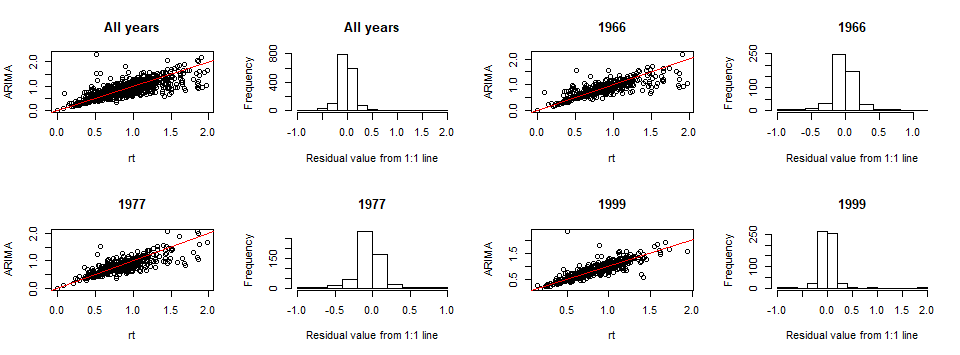
\includegraphics{tables_figures/publication/figureS4_Rt_arima_comparison.png}
\caption{Figure S4}
\end{figure}

\textbf{Regarding the resilience indices, we considered analyzing these
and decided it would be best to stick with just resistance for three
reasons: (1) Most importantly, we would expect resilience to be governed
by fundamentally different mechanisms than resistance. While it would be
interesting to examine resilience, this would be beyond the scope of the
current paper. (2)
\href{https://www.nature.com/articles/s41467-020-14300-5}{DeSoto et
al.~(2020, Nature)} used an extensive dataset of trees sampled after
severe droughts and compared the responses to previous, less-severe
droughts between trees that survived and trees that were killed by the
severe drought. In angiosperms, trees that died from a severe drought
had lower resistance to previous droughts, compared to trees that
survived the severe drought. In gymnosperms, trees that died during
severe droughts had lower recovery following previous droughts, compared
to trees that survived the severe drought. These findings would argue
that resistance is a more important variable for angiosperms. We now
state the logic for focusing on \(Rt\) in the methods section:}

\textbf{``We focus exclusively on drought resistance (\(Rt\) or
\(Rt_{ARIMA}\)), and not on the resilience metrics described in Lloret
\emph{et al.} (2011), because (1) we would expect resilience to be
controlled by a different set of mechanisms, and (2) the findings of
\emph{\href{https://www.nature.com/articles/s41467-020-14300-5}{DeSoto
et al.~(2020)}} suggest that \(Rt\) is a more important drought response
metric for angiosperms.''}

Secondly, the choice of traits does not appear well justified, as it
seems to be driven more by easiness of measurement than by relevance,
and it mixes different types of hypotheses operating at different
levels. On one hand there is tree height and crown position, which are
measured at the level of individual trees and correspond to closely
related hypotheses. On the other hand there are ring-porosity, wood
density, LMA and water relations traits, which are measured at the
species level and seem to be totally disconnected from the hypotheses
regarding tree height. In addition, it is very hard to compare the
explanatory power of these variables, as done in the paper, as they are
based on very different sample sizes (571 trees vs 12 species) and
respond to different sources of variability. In fact the way height
effects are analyzed mixes the within- and between-species levels, which
makes it difficult to interpret the results. Finally, I think it would
be more correct to refer to PLA and TLP as water relations traits rather
than hydraulic traits.

Thirdly, a more thorough analysis of the distribution of the study
species in the sample plot would be required. The paper assumes that all
species were subjected to the same drought levels. However, this is
unlikely to be true, as different species are likely to occupy different
microhabitats in the plot, and hence be subjected to different drought
conditions. The authors account for this, to some extent, by including
individual-level TWI in some models, but a more thorough analysis of the
distribution of the study species as a function of TWI and other
relevant micro-environmental variables would be needed to fully
interpret the results.

\emph{It seems from these comments they think this shouldn't be
published at all due to its limited scope and not enough explanatory
power. The resulting study that they suggest, if completely thorough,
would take a long time to create. I'm not sure how to address this
comment, other than to make a note in the manuscript acknowledging that
a more thorough study would be great but this is what we found with what
we had.}

\emph{I agree\ldots. I wouldn't change analysis for this. We can come
back to wording a response later.}

Minor or more technical suggestions:

L59-79: the arguments presented in this paragraph mix different scales,
from within-individual to within- or among-communities. I think the
arguments could be better structured to reflect the sources of
variability involved and, ideally, focus on the scale that will be
addressed in the paper.

L67: I suggest toning down the sentence to something like `Wider xylem
conduits are associated to higher vulnerability to embolism during
drought', as the mechanism linking wider conduits with embolism
vulnerability is far from clear and probably indirect.

L81: you seem to use drought resistance and drought tolerance
interchangeably, which may be confusing. I think it is important to
clarify these definitions early on in the paper.

L97: `greater variation' that what?

L100-101: that is not true really. See for example Zhu et al.~(2018) in
Tree Phys, Farrell et al.~(2017) in PCE\ldots{}

L137-140: mixing cores from dying and surviving individuals could be
problematic. Did you find any association between survival and previous
drought resistance? Was mortality different across species?

L160: you mean a log-log regression, right?

L181: N=3 individuals per species is really quite low. In addition, by
sampling up to 8 m height you would probably be sampling less exposed
branches from taller trees, which could confound your results.

\emph{from NObby: ``Regarding the few individuals I would argue that
intraspecific SD was low (less than 10\% of the mean values). This
justifies - in my opinion - only sampling three individuals.''}

L188: `Wood'.

\textbf{Fixed.}

L189: fresh volume?

\textbf{Yes, now specified.}

L223: clarify that the -4.53 value corresponds to July.

L228-234: please clarify model structure. I understand you included tree
as a random factor only when the three droughts were analyzed together,
right? It would be nice to know what was the contribution of random
factors to model fit (only one R2 is shown in Table 5, and it is unclear
whether it corresponds to marginal or conditional values).

L238, 242, 244: it is unclear to me why in some cases you use a dAICc of
1 and sometimes of 2.

L287-299: it would be very useful to use scatterplots to show the
effects of traits on Rt in a figure.

\href{https://github.com/SCBI-ForestGEO/McGregor_climate-sensitivity-variation/issues/71}{\emph{issue
\#71}}

L291-294: but this is problematic considering that you only had two
diffuse-porous species.

\textbf{We have made changes to the analysis that resulted in dropping
ring porosity from the full models. While we agree that it is
problematic that we only have two ring-porous species, we believe that
it's worth including because this engages with, and rejects, the
existing understanding that in this biome, ring-porous species are more
drought tolerant.}

L297: TLP was significant for 1966 according to Table 4.

L301-302: I would tone down this, as your models explained a rather low
\% of the variation in Rt.

L305-306: not for the 1977 and 1999 droughts, according to Table 5.

L314-316: or simply that your sample size was rather low. See also main
comments above.

L329-331: do you have any information on the demographic effects (e.g.,
mortality) of the three droughts studied?

\textbf{Unfortunately, no. All we could say is that the 1999 drought
didn't result in a big loss of live biomass.}

Table 3: are DBH units correct? I suspect they should be mm instead of
cm.

\emph{These are incorrect. Ian, please convert to cm.}

Figure 1: please explain all acronyms.

\textbf{We now specify that these codes are given in Table 3.}

Figure 2: where are the leaf hydraulic traits shown (cf.~caption)?

\textbf{It was an error that this was mentioned in the caption; now
removed.}

Table S1: why only 11 species? Some of the fits are really low\ldots{}

\textbf{Bark thickness measurements were drawn from an existing data
set, and we did not make additional measurements because the trait is
unlikely to have meaningful influence on results. This study already
goes above and beyond the existing norm for accounting for bark
thickness in DBH reconstructions; typically there is no correction for
changes in bark thickness as the tree ages.}

Table S3: what does `rank' refer to?

\textbf{This has been clarified.}

Figure S1: please add spatial scale to the figure.

\emph{IAN, please do this}

Figure S3: please specify that height values are estimated from
reconstructed DBH.

\textbf{Done.}

\hypertarget{citations}{%
\subsection*{Citations}\label{citations}}
\addcontentsline{toc}{subsection}{Citations}

\hypertarget{refs}{}
\leavevmode\hypertarget{ref-bennett_larger_2015}{}%
\textbf{\textnormal{Bennett AC}, \textnormal{McDowell NG},
\textnormal{Allen CD}, \textnormal{Anderson-Teixeira KJ}}.
\textbf{2015}. Larger trees suffer most during drought in forests
worldwide. \emph{Nature Plants} \textbf{1}: 15139.

\leavevmode\hypertarget{ref-elliott_forest_2015}{}%
\textbf{\textnormal{Elliott KJ}, \textnormal{Miniat CF},
\textnormal{Pederson N}, \textnormal{Laseter SH}}. \textbf{2015}. Forest
tree growth response to hydroclimate variability in the southern
Appalachians. \emph{Global Change Biology} \textbf{21}: 4627--4641.

\leavevmode\hypertarget{ref-friedrichs_species-specific_2009}{}%
\textbf{\textnormal{Friedrichs DA}, \textnormal{Trouet V},
\textnormal{Büntgen U}, \textnormal{Frank DC}, \textnormal{Esper J},
\textnormal{Neuwirth B}, \textnormal{Löffler J}}. \textbf{2009}.
Species-specific climate sensitivity of tree growth in Central-West
Germany. \emph{Trees} \textbf{23}: 729.

\leavevmode\hypertarget{ref-helcoski_growing_2019}{}%
\textbf{\textnormal{Helcoski R}, \textnormal{Tepley AJ},
\textnormal{Pederson N}, \textnormal{McGarvey JC}, \textnormal{Meakem
V}, \textnormal{Herrmann V}, \textnormal{Thompson JR},
\textnormal{Anderson‐Teixeira KJ}}. \textbf{2019}. Growing season
moisture drives interannual variation in woody productivity of a
temperate deciduous forest. \emph{New Phytologist} \textbf{0}.

\leavevmode\hypertarget{ref-kannenberg_linking_2019}{}%
\textbf{\textnormal{Kannenberg SA}, \textnormal{Novick KA},
\textnormal{Alexander MR}, \textnormal{Maxwell JT}, \textnormal{Moore
DJP}, \textnormal{Phillips RP}, \textnormal{Anderegg WRL}}.
\textbf{2019}. Linking drought legacy effects across scales: From leaves
to tree rings to ecosystems. \emph{Global Change Biology} \textbf{0}.

\leavevmode\hypertarget{ref-liu_hydraulic_2019}{}%
\textbf{\textnormal{Liu H}, \textnormal{Gleason SM}, \textnormal{Hao G},
\textnormal{Hua L}, \textnormal{He P}, \textnormal{Goldstein G},
\textnormal{Ye Q}}. \textbf{2019}. Hydraulic traits are coordinated with
maximum plant height at the global scale. \emph{Science Advances}
\textbf{5}: eaav1332.

\leavevmode\hypertarget{ref-lloret_components_2011}{}%
\textbf{\textnormal{Lloret F}, \textnormal{Keeling EG}, \textnormal{Sala
A}}. \textbf{2011}. Components of tree resilience: Effects of successive
low-growth episodes in old ponderosa pine forests. \emph{Oikos}
\textbf{120}: 1909--1920.

\leavevmode\hypertarget{ref-olson_plant_2018}{}%
\textbf{\textnormal{Olson ME}, \textnormal{Soriano D},
\textnormal{Rosell JA}, \textnormal{Anfodillo T}, \textnormal{Donoghue
MJ}, \textnormal{Edwards EJ}, \textnormal{León-Gómez C},
\textnormal{Dawson T}, \textnormal{Martínez JJC}, \textnormal{Castorena
M} \emph{et al.}} \textbf{2018}. Plant height and hydraulic
vulnerability to drought and cold. \emph{Proceedings of the National
Academy of Sciences} \textbf{115}: 7551--7556.

\leavevmode\hypertarget{ref-stovall_tree_2019}{}%
\textbf{\textnormal{Stovall AEL}, \textnormal{Shugart H},
\textnormal{Yang X}}. \textbf{2019}. Tree height explains mortality risk
during an intense drought. \emph{Nature Communications} \textbf{10}:
1--6.

\leavevmode\hypertarget{ref-zuleta_drought-induced_2017}{}%
\textbf{\textnormal{Zuleta D}, \textnormal{Duque A},
\textnormal{Cardenas D}, \textnormal{Muller‐Landau HC},
\textnormal{Davies SJ}}. \textbf{2017}. Drought-induced mortality
patterns and rapid biomass recovery in a terra firme forest in the
Colombian Amazon. \emph{Ecology} \textbf{98}: 2538--2546.

\end{document}
